\documentclass{ccnudoc}
\usepackage{multirow, xeCJKfntef, xpinyin}
\usepackage{graphicx}
\usepackage{tabularray}
\usepackage[
  backend = biber,
  style = gb7714-2015
]{biblatex}
\addbibresource{CCNUthesis.bib}
\graphicspath{{figures}}

\hypersetup{
  pdftitle  = {CCNUthesis: 华中师范大学学位论文模版},
  pdfauthor = {夏康玮}
}
% 全角标点放在引号中,需要改成半角式,否则间距过大,不好看
\def\FSID{“{\xeCJKsetup{PunctStyle=banjiao}。}”} % U+3002
\def\FSFW{“{\xeCJKsetup{PunctStyle=banjiao}.}”} % U+FF0E
\def\COFW{“{\xeCJKsetup{PunctStyle=banjiao}:}”} % U+FF1A
\def\SCFW{“{\xeCJKsetup{PunctStyle=banjiao};}”} % U+FF1B


\title{\textcolor{MaterialIndigo800}{%
  \textbf{CCNUthesis: 华中师范大学学位论文\xpinyin[font=\sffamily,format=\color{MaterialIndigo800}]{模}{mu2}板}}}
\author{夏康玮}
\date{2022/06/04\quad v1.2.4%
  \thanks{%
    \parbox{0.5\textwidth}{
      \url{https://github.com/xkwxdyy/CCNUthesis} \\
      \url{https://gitee.com/xkwxdyy/CCNUthesis}
    }
  }
}


\begin{document}
\newgeometry{
  left   = 2.2 in,
  right  = 1.25 in,
  top    = 1.25 in,
  bottom = 1.00 in
}

\maketitle

\begin{abstract}
华中师范大学学位论文 \LaTeX{} 模板 \cls{CCNUthesis} 基于本科生院的论文撰写规范制作,同时参考研究生院提供的《研究生学位论文规范》,用于生成符合华中师范大学学位论文排版要求和相应的国家规范、行业标准的学位论文,旨在为同学提供毕业论文书写的方便。
\end{abstract}

\def\abstractname{Abstract}
\begin{abstract}
The \cls{CCNUthesis} class is intended for typesetting Central China Normal University dissertations with \LaTeX{}, providing support for bachelor, master, and doctoral thesis.
\end{abstract}

\vspace{2cm}
\def\abstractname{特别声明}
\begin{abstract}
在使用本模板时,我们默认您同意以下内容:
\begin{enumerate}
  \item 本模板通过 LPPL 1.3c 协议开放源代码,您可以随意使用编译出的 PDF 文件。
  \item 本模板与学校官方部门并不存在合作关系,作者不对使用本模板产生的格式审查问题负责。
  \item 遇到本文档没有覆盖的问题属于正常情况,欢迎提交反馈意见。
\end{enumerate}
\end{abstract}

\begin{tikzpicture}[remember picture, overlay]
  \node[opacity = 0.1] at ([shift={(0.1\textwidth, -0.45\textheight)}]current page text area.north west){
    
\includegraphics[width=26cm]{ccnu-logo.png}
  };
\end{tikzpicture}
\thispagestyle{plain}
\clearpage


% 用户手册的页边距

\newgeometry{
  left   = 1.65 in,
  right  = 0.80 in,
  top    = 1.25 in,
  bottom = 1.00 in
}

\tableofcontents



\section{介绍} 

目前,在网上可以找到的华中师范大学 \LaTeX{} 论文模板主要是

\begin{itemize}
  \item 由华中师范大学数学与统计学学院邓国泰老师编写的本科毕业论文模版
  \item 华中师范大学数学与统计学学院基础数学方向“流传”下来的硕士模版
\end{itemize}

但这些模板基于 \CTeX 套装编写, \CTeX 套装已经近十年未更新,已不能适应当前 \TeX{} 中文技术的发展,引用 \CTeX 套装的开发之一刘海洋的话:\emph{\CTeX 已经完成了它的历史使命。} 更多关于不推荐使用 \CTeX 套装的原因参看 \href{https://gitee.com/xkwxdyy/CCNUthesis/wikis/%E5%B8%B8%E8%A7%81%E9%97%AE%E9%A2%98FAQ/%E4%B8%BA%E4%BB%80%E4%B9%88%E4%B8%8D%E6%8E%A8%E8%8D%90%E5%AE%89%E8%A3%85\CTeX%E5%A5%97%E8%A3%85%E4%BA%86}{《为什么不推荐安装 \CTeX 套装了》}。

抛开旧模版是基于 \CTeX 套装编写的这一点,关于旧模版本身也有众多使用问题,比如格式相关代码不能完全剥离,导致用户,尤其是 \LaTeX{} 初学者,使用起来体验不佳。笔者整理过邓国泰老师编写的本科毕业论文模版中出现的问题,并对照着阐述了新模版的优化处理,感兴趣的用户可以参看 \href{https://gitee.com/xkwxdyy/CCNUthesis/wikis/%E5%B8%B8%E8%A7%81%E9%97%AE%E9%A2%98FAQ/%E6%97%A7%E6%A8%A1%E7%89%88%E7%9A%84%E4%BD%BF%E7%94%A8%E6%96%B9%E5%BC%8F%E6%9C%89%E4%BB%80%E4%B9%88%E9%97%AE%E9%A2%98%EF%BC%9F%E6%96%B0%E6%A8%A1%E7%89%88%E7%9A%84%E4%BD%BF%E7%94%A8%E6%98%AF%E5%A6%82%E4%BD%95%E5%AE%8C%E5%96%84%E7%9A%84%EF%BC%9F}{《旧模版的使用方式有什么问题?新模版的使用是如何完善的?》}。

相比之下,复旦大学 \cls{CCNUthesis}、清华大学 \cls{thuthesis}、中国科学技术大学 \cls{ustcthesis}、中国科学院大学 \cls{ucasthesis} 以及上海交通大学 \cls{sjtuthesis} 等学位论文 \LaTeX{} 模版成熟稳定,值得参考。

本模板将借鉴前辈经验,重新设计,并使用 \LaTeX3 编写,以适应 \TeX{} 技术发展潮流;同时还将构建一套简洁的接口,方便用户使用。


\subsection{\TeXLive 安装}

要想使用 \LaTeX{} 及此模板,必须安装 \TeXLive 发行版,安装介绍只推荐啸行编写的 \href{https://ctan.math.illinois.edu/info/install-latex-guide-zh-cn/install-latex-guide-zh-cn.pdf}{install-latex-guide-zh-cn},关于此文档的一些补充,参看 \href{https://gitee.com/xkwxdyy/CCNUthesis/wikis/%E5%B8%B8%E8%A7%81%E9%97%AE%E9%A2%98FAQ/%E5%A6%82%E4%BD%95%E5%AE%89%E8%A3%85TeXLive}{《如何安装 TeXLive ?》}。


\subsection{\LaTeX{} 入门}

本文档并非是一份 \LaTeX{} 零基础教程。如果您是完完全全的新手,建议先阅读相关入门文档,虽然网络上的入门教程多如牛毛,但是强烈建议阅读 \href{https://ctan.math.illinois.edu/info/lshort/chinese/lshort-zh-cn.pdf}{lshort-zh-cn},并且用好 \cmd{texdoc} 命令(lshort-zh-cn 中有介绍)查看相关宏包手册进行更全面的学习。


\subsection{关于本文档} \label{subsec:提issues}

本文采用不同字体表示不同内容。无衬线字体表示宏包名称,如
\pkg{xeCJK} 宏包、\cls{CCNUthesis} 文档类等;等宽字体表示代码或
文件名,如 \cs{ccnusetup} 命令、\env{abstract} 环境、\TeX{} 文档
\file{main.tex} 等;带有尖括号的楷体(或西文斜体)表示命令参数,
如 \meta{模板选项}、\meta{English title} 等。在使用时,参数两侧
的尖括号不必输入。示例代码进行了语法高亮处理,以方便阅读。

在用户手册中,带有蓝色侧边线的为 \LaTeX{} 代码,而带有粉色侧边线
的则为命令行代码,请注意区分。模板提供的选项、命令、环境等,
均用横线框起,同时给出使用语法和相关说明。

% 本模板中的选项、命令或环境可以分为以下三类:
% \begin{itemize}
%   \item 名字后面带有 \rexptarget\rexpstar{} 的,表示只能
%     在\emph{中文模板}中使用;
%   \item 名字后面带有 \exptarget\expstar{} 的,表示只能
%     在\emph{英文模板}中使用;
%   \item 名字后面不带有特殊符号的,表示既可以在中文模板中使用,
%     也可以在英文模板中使用。
% \end{itemize}

如果您有任何改进意见或者功能需求,欢迎前往 \href{https://github.com/xkwxdyy/CCNUthesis/issues}{gitHub 仓库 issues} 或 \href{https://gitee.com/xkwxdyy/CCNUthesis/issues}{gitee 仓库 issues} 提交 issue。



\section{安装}

\subsection{获取 \cls{CCNUthesis}}

目前模块还处于刚开发完的阶段,决定暂时用户以「下载发行版」的方式获取最新版本的 \cls{CCNUthesis}:

\begin{enumerate}
  \item 进入项目主页(\href{https://github.com/xkwxdyy/CCNUthesis}{github 项目主页} (界面见图~\ref{figure:github项目主页} )或 \href{https://gitee.com/xkwxdyy/CCNUthesis}{gitee 项目主页} (界面见图~\ref{figure:gitee项目主页} ))
  \item 在右侧一列有“发行版”(gitee)或“Releases”(github),并且有一个标签图标并有“vx.x.x - 20xx-xx-xx”字样,表示最新的发行版版本和发布时间,点击即可查看相关信息(如果想查看历史所有发行版信息,可以点击“Releases”(github)或“发行版”右侧的“全部”(gitee))。
  
    发行版中一般由以下信息构成(\href{https://github.com/xkwxdyy/CCNUthesis/releases}{github 发行版} 界面见图~\ref{figure:github发行版},\href{https://gitee.com/xkwxdyy/CCNUthesis/releases}{gitee 发行版} 界面见图~\ref{figure:gitee发行版})
      \begin{itemize}
        \item 更新文件的特别说明。如果没有,则表明此次更新只需要更新 \file{CCNUthesis.cls} 文件至最新\footnote{“更新 \meta{文件} 至最新”目前表示在发行版中下载最新版本的模板,并用其中所需要更新的 \meta{文件} 去替换本地的旧 \meta{文件}} 即可
        \item 更新日志。主要为此次发行版与上次发行版的不同,比如“Added”、“Changed”、“Fixed”等等信息
        \item 模版及用户手册下载链接。github 的为“Assets”部分,gitee 的为“下载”部分。一般用户只需要点击 \file{CCNUthesis-vx.x.x.zip} 进行模版下载即可,而下面的 \file{Source code} 为项目的整个源码,包括手册的源码,测试文件等,如果感兴趣的用户可以下载进行查看(当然,如果会使用 \cmd{git} 的用户也可以将整个 \cls{CCNUthesis} 项目 \cmd{clone} 下来查看)
      \end{itemize}
  \item 点击 \file{CCNUthesis-vx.x.x.zip} 进行下载,在本地解压即可
\end{enumerate}

\begin{figure}[htbp]
  \centering
  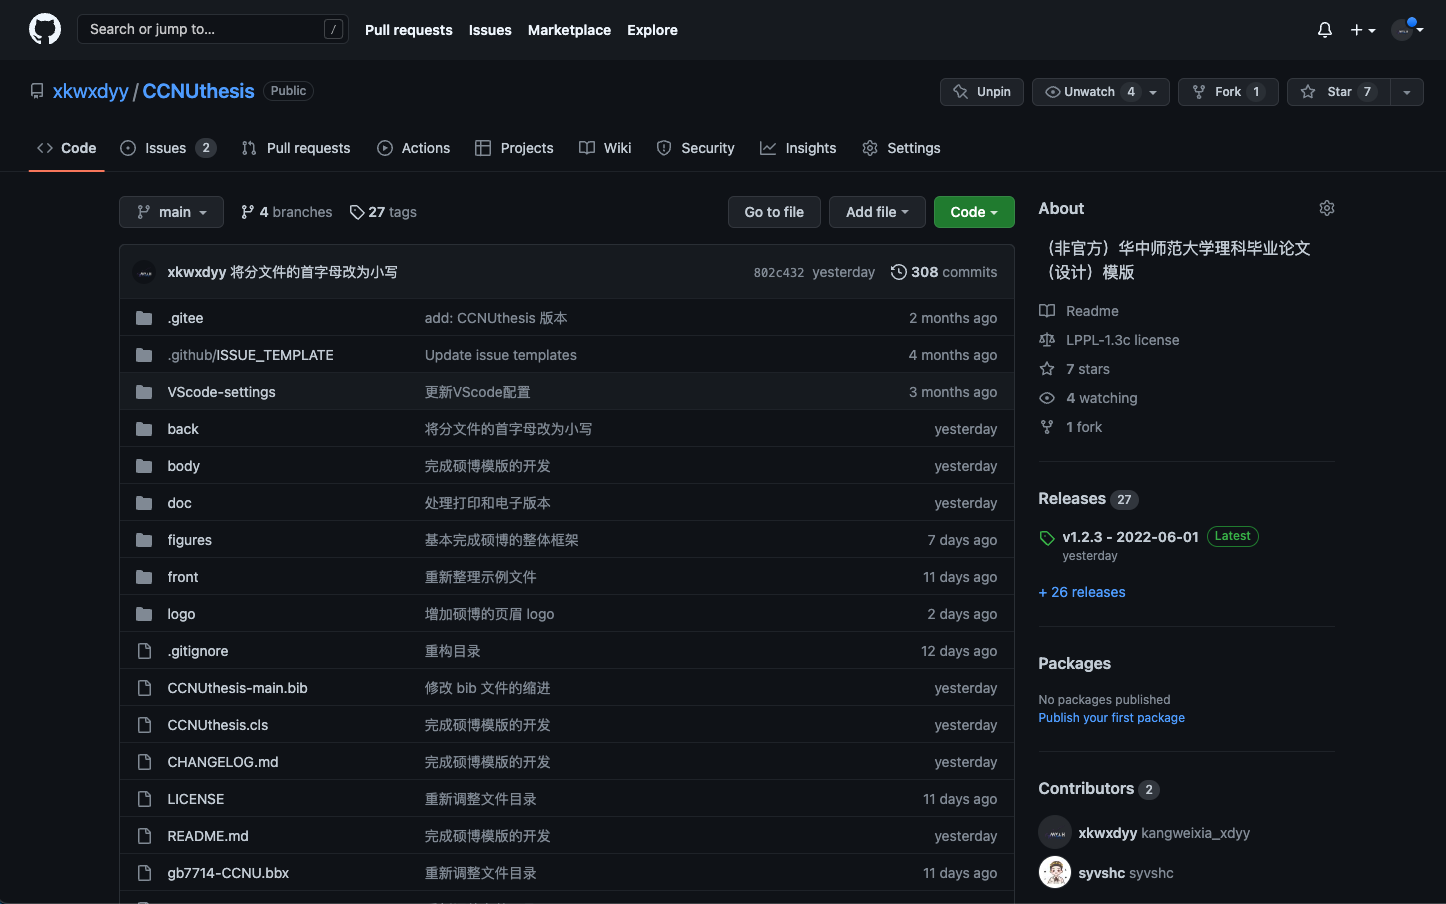
\includegraphics[width = \textwidth]{github项目主页.png}
  \caption{github 项目主页}
  \label{figure:github项目主页}
\end{figure}

\begin{figure}[htbp]
  \centering
  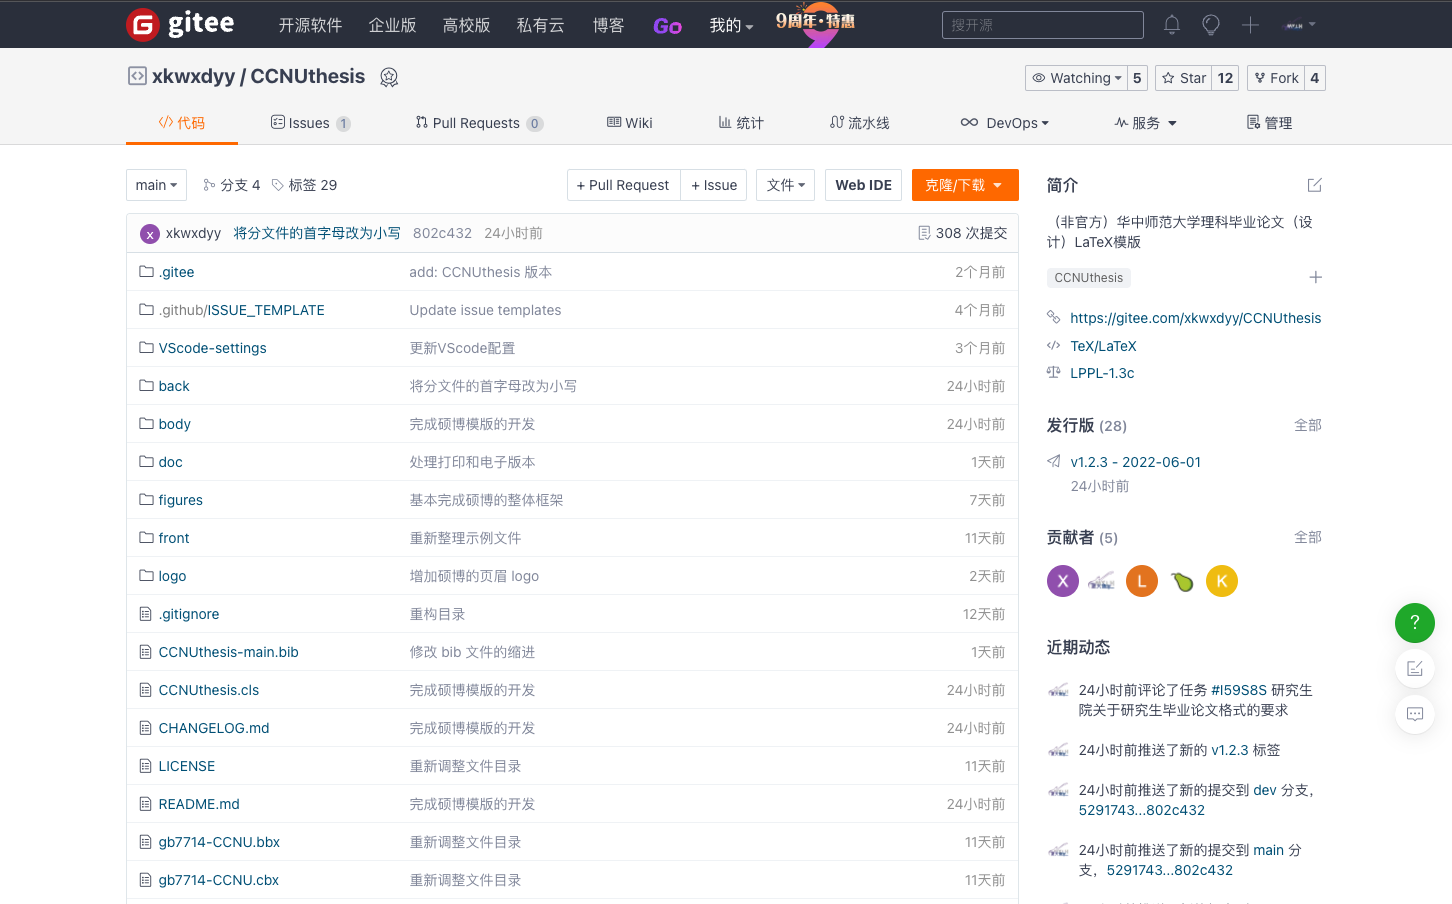
\includegraphics[width = \textwidth]{gitee项目主页.png}
  \caption{gitee 项目主页}
  \label{figure:gitee项目主页}
\end{figure}


\begin{figure}[htbp]
  \centering
  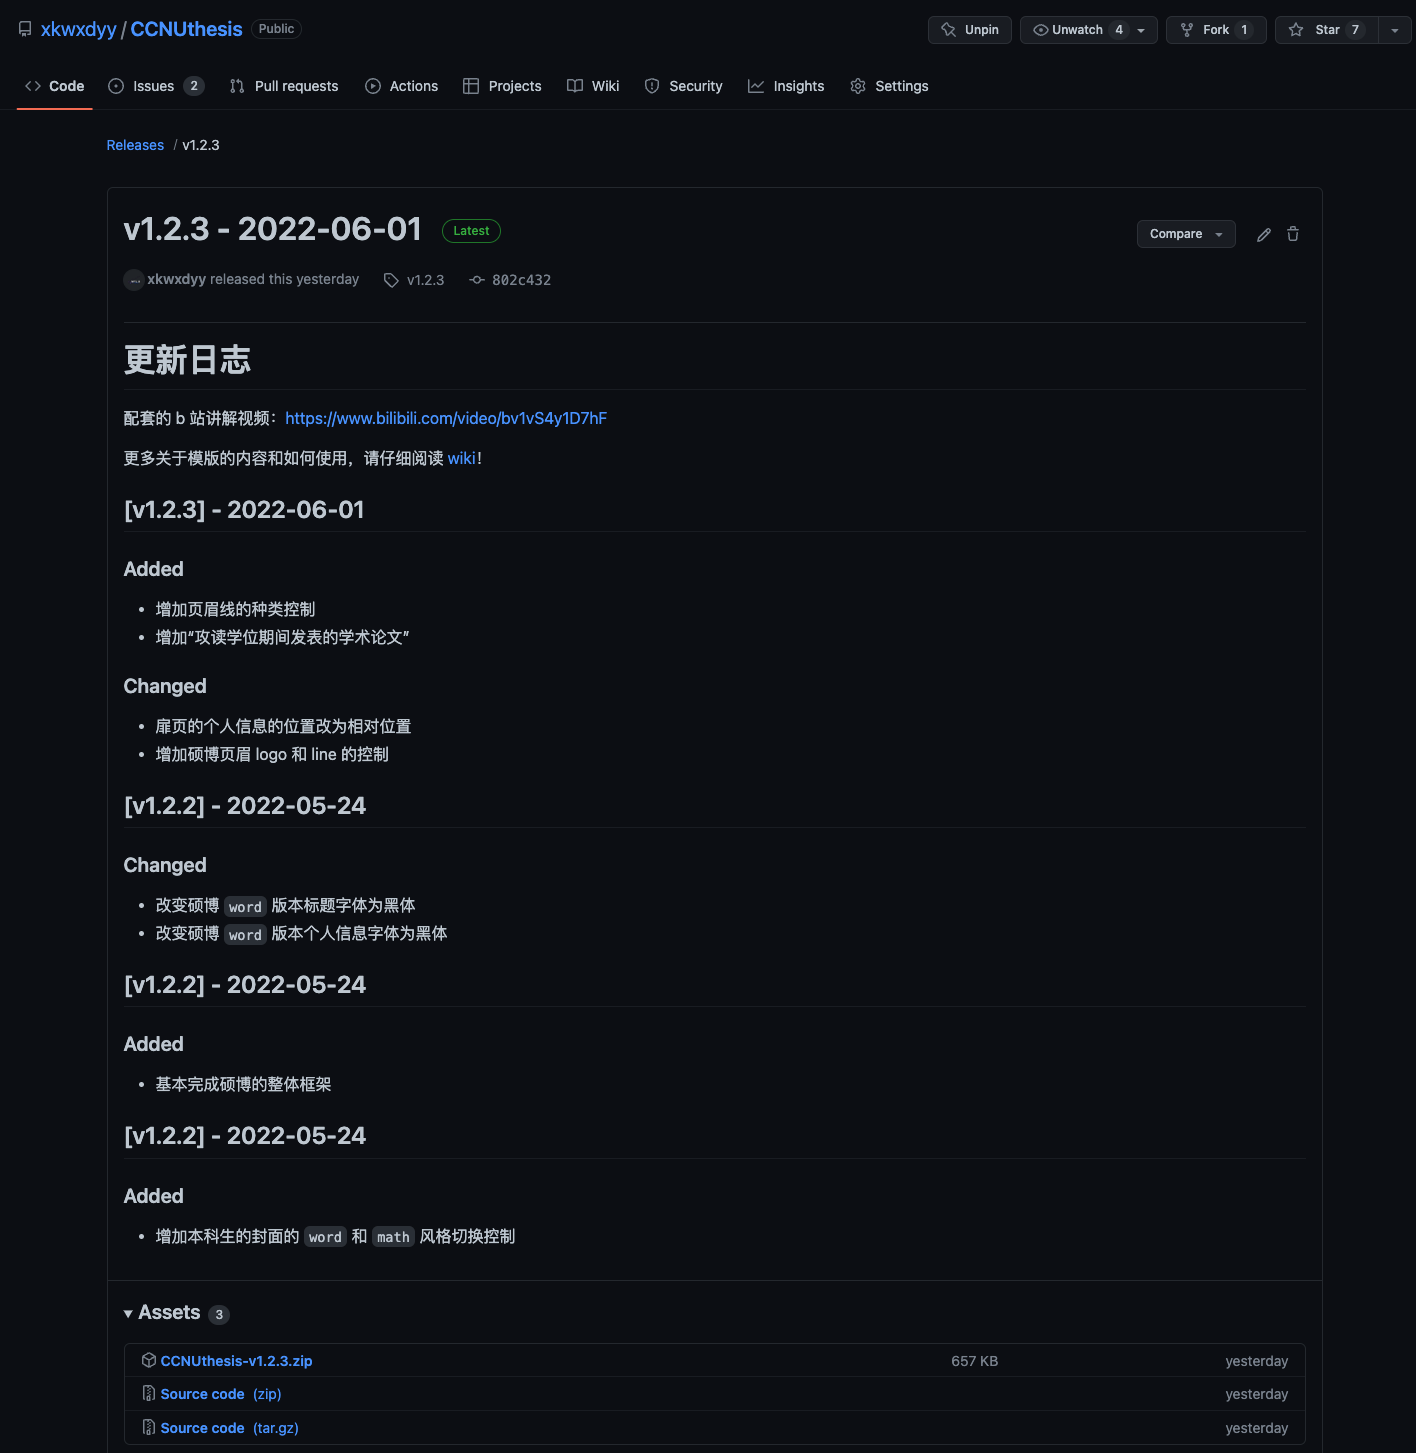
\includegraphics[width = \textwidth]{github发行版.png}
  \caption{github 发行版}
  \label{figure:github发行版}
\end{figure}

\begin{figure}[htbp]
  \centering
  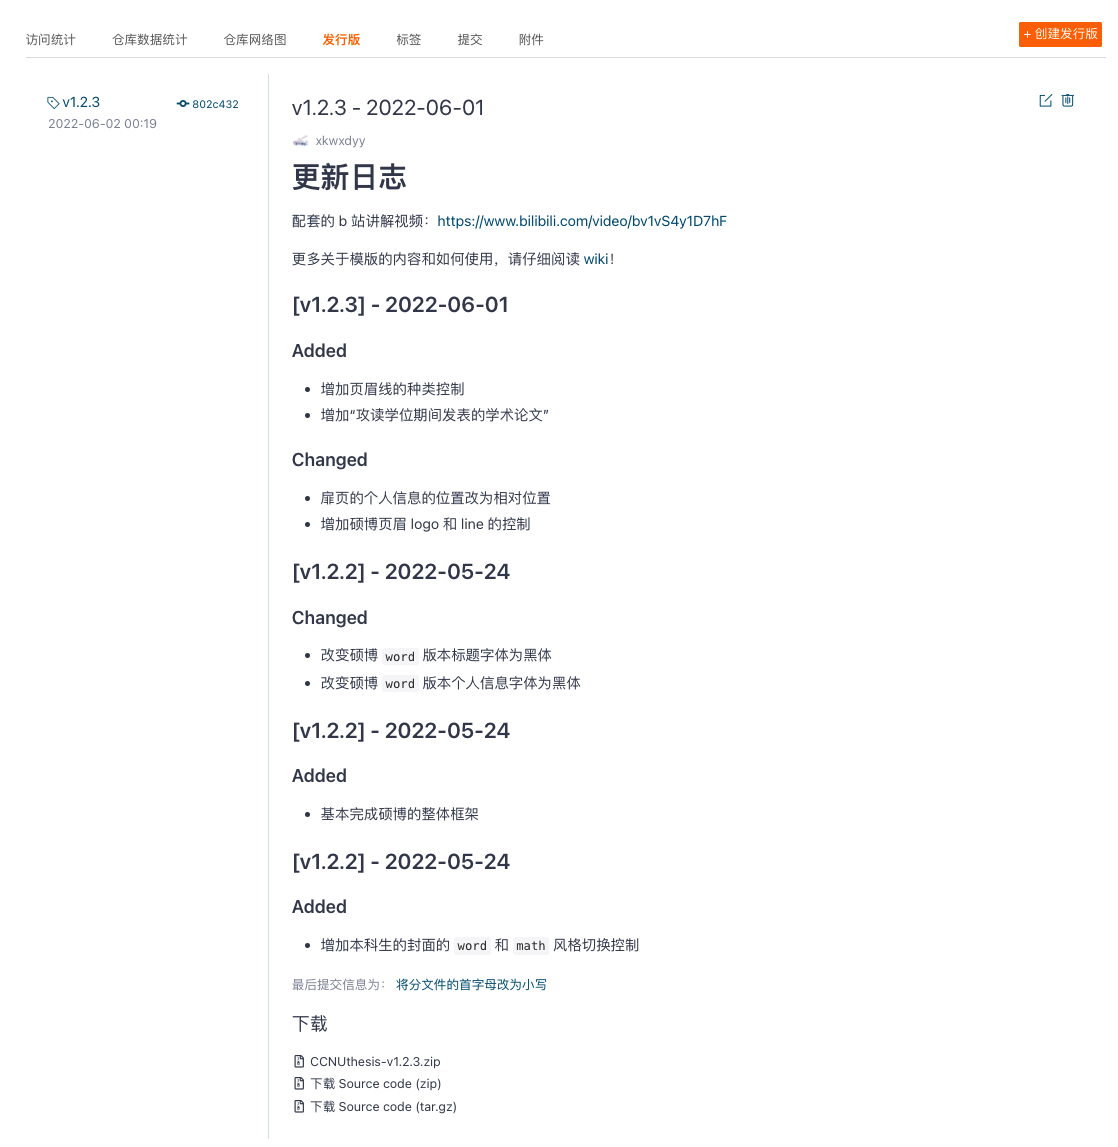
\includegraphics[width = \textwidth]{gitee发行版.png}
  \caption{gitee 发行版}
  \label{figure:gitee发行版}
\end{figure}

% \subsubsection{标准安装}

% 如果没有特殊理由,始终建议您使用宏包管理器安装 \cls{CCNUthesis}。
% 例如在 \TeXLive{} 中,执行(可能需要管理员权限)
% \begin{shellexample}[morekeywords={tlmgr,install}]
%   tlmgr install CCNUthesis
% \end{shellexample}
% 即可完成安装。

% 在 \TeXLive{} 和 \MiKTeX{} 中,您还可以通过图形界面进行安装,
% 此处不再赘述。

% \subsubsection{手动安装}

% 如果您需要从 CTAN 上自行下载并手动安装,较好的方法是使用 TDS
% 安装包:
% \begin{itemize}
%   \item 从 CTAN 上下载 \cls{CCNUthesis} 的
%     \href{http://mirror.ctan.org/install/macros/latex/contrib/CCNUthesis.tds.zip}{TDS 安装包};
%   \item 按目录结构将 \file{CCNUthesis.tds.zip} 中的文件复制到 \TeX{}
%     发行版的本地 TDS 根目录;
%   \item 执行 \bashcmd{mktexlsr} 刷新文件名数据库以完成安装。
% \end{itemize}
% %
% 您也可以从源代码直接生成模板(不推荐):
% \begin{itemize}
%   \item 打开 \href{https://github.com/stone-zeng/CCNUthesis}{项目主页},
%     点击“Code”按钮,并选择“Download ZIP”,下载 \file{CCNUthesis-main.zip};
%     如果您的电脑中安装有 git 程序,也可通过以下命令直接克隆代码仓库:
%     \begin{shellexample}[gobble=6,alsoletter={.},morekeywords={git,clone}]
%       git clone https://github.com/stone-zeng/CCNUthesis.git
%     \end{shellexample}
%   \item 解压并进入到 \file{source} 文件夹,执行以下命令以生成
%     模板的各组件:
%     \begin{shellexample}[gobble=6,morekeywords={xetex}]
%       xetex CCNUthesis.dtx
%     \end{shellexample}
%   \item 将生成的文档类(\file{.cls})、宏包(\file{.sty})以及
%     参数配置文件(\file{.def})复制到 \TeX{} 发行版本地 TDS 树
%     的 \path{texmf-local/tex/latex/CCNUthesis/} 目录下,并执行
%     \bashcmd{mktexlsr} 刷新文件名数据库,方可完成安装。
%   \item 使用 \cls{CCNUthesis} 撰写论文时,您还需要从代码仓库下的
%     \file{testfiles/support} 目录中复制 \file{fudan-name.pdf}
%     文件至工作目录,以确保封面中的校名图片可以正确显示。
% \end{itemize}

% \subsubsection{扁平化安装}

% 如果您不希望安装本模板,但需要立刻使用,也可以使用模板提供的安装脚本。
% 从 GitHub 上获取代码仓库后,执行 \file{install-win.bat}(Windows 系统)
% 或 \file{install-linux.sh}(Linux 系统),所有需要的文件便会在
% \file{thesis} 文件夹中生成。


\subsection{模板组成}

本模板主要包含核心文档类、参考文献格式文件以及用户文档等几个部分,
其具体组成见表~\ref{tab:ccnuthesis-main-components},模版子目录中的文件组成见表~\ref{tab:ccnuthesis-sub-components}。

\begin{table}[htbp]
  \caption{\cls{CCNUthesis} 的主要组成部分}
  \label{tab:ccnuthesis-main-components}
  \centering
  \small
  \begin{tblr}{
    hline{1, 2, Z} = {1pt},
    width = \textwidth,
    colspec = {X[2,l]X[5,l]},
    rows = {m}
  }
    \textbf{文件} & \textbf{功能说明} \\
    \file{CCNUthesis.pdf}         & 用户手册(本文档) \\
    \file{main.tex}               & 模板的主文件,可据此为基础完成论文撰写 \\
    \file{CCNUthesis.cls}         & 模板文档类 \\
    \file{CCNUthesis-main.bib}    & 参考文献数据库文件,里面的条目均为示例,可删除后输入用户自己的参考文献条目并在正文中进行引用 \\
    {\file{gb7714-CCNU.bbx} \\ \file{gb7714-CCNUay.bbx}} & 参考文献的条目格式文件 \\
    \file{gb7714-CCNU.cbx}        & 参考文献的引用格式文件 \\
    \file{latexmkrc}              & \pkg{latexmk} 编译命令的配置文件 \\
    \file{README.md}              & 简要自述 \\
    \file{CHANGELOG.md}           & 模板更新日志 \\
    \file{LICENSE}                & 模版发布许可证
  \end{tblr}
\end{table}

\begin{table}[htbp]
  \caption{\cls{CCNUthesis} 各目录的组成部分}
  \label{tab:ccnuthesis-sub-components}
  \centering
  \small
  \begin{tblr}{
    hline{4,5,8,11,13} = {solid},
    hline{1, 2, Z} = {1pt},
    width = \textwidth,
    colspec = {X[1,l]X[3,l]X[3,l]},
    rows = {m},
    cell{2}{1} = {r=2}{m},
    cell{5}{1} = {r=3}{m},
    cell{8}{1} = {r=3}{m},
    cell{11}{1} = {r=2}{m},
  }
    \textbf{子目录} & \textbf{子目录中的文件} & \textbf{功能说明} \\
    front & \file{abstract.tex}            & 中英文摘要 \\
    front & \file{notation.tex}            & 符号表 \\
    body  & \file{chapter<number>.tex}     & 正文的分文件 \\
    back  & \file{acknowledgements.tex}    & 致谢 \\
    back  & \file{appendix.tex}            & 附录 \\
    back  & \file{publications.tex}        & 攻读学位期间取得的研究成果(博士)\\
    logo  & \file{ccnulogo.png}            & “华中师范大学”字样 logo \\
    logo  & \file{masterlogo.png}          & 硕士学位论文页眉 logo \\
    logo  & \file{doctorlogo.png}          & 博士学位论文页眉 logo \\
    copyright  & \file{Originality_Copyright.pdf}  & 本科学位论文原创性声明和使用授权说明 \\
    copyright  & \file{Originality_Copyright_master_doctor.pdf}  & 硕博学位论文原创性声明和使用授权说明\\
    figures & & 用户放置图片的目录\\
  \end{tblr}
\end{table}



\section{使用说明}

\subsection{基本用法}

以下是一份简单的 \TeX{} 文档,它演示了 \cls{CCNUthesis} 的最基本用法:

\begin{latexexample}[deletetexcs={\documentclass},
    moretexcs={\chapter},morekeywords={\documentclass},
    emph={[2]document}]
  % main.tex
  \documentclass{CCNUthesis}
  \begin{document}
    \chapter{欢迎}
    \section{Welcome to CCNUthesis!}
    你好,\LaTeX{}!
  \end{document}
\end{latexexample}


按照~\ref{subsec:编译方式} 小节中的方式编译该文档,您应当得到一篇 3 页的文章。

% 英文模板可以用类似的方式使用:

% \begin{latexexample}[deletetexcs={\documentclass},
%     moretexcs={\chapter},morekeywords={\documentclass},
%     emph={[2]document}]
%   % thesis-en.tex
%   \documentclass{CCNUthesis-en}
%   \begin{document}
%     \chapter{Welcome}
%     \section{Welcome to CCNUthesis!}
%     Hello, \LaTeX{}!
%   \end{document}
% \end{latexexample}

% 英文模板只对正文部分进行了改动,封面、指导小组成员以及声明页仍将
% 显示为中文。

\subsection{编译方式} \label{subsec:编译方式}

本模板不支持 \pdfTeX{} 引擎,仅支持使用 \XeLaTeX{} 。为了生成正确的目录、脚注以及交叉引用,您至少需要连续编译两次。

以下代码中,假设您的 \TeX{} 源文件名为 \file{main.tex}。请在命令行中执行
\begin{shellexample}[morekeywords={xelatex}]
  xelatex main
\end{shellexample}
或使用 \pkg{latexmk}:
\begin{shellexample}[morekeywords={latexmk},emph={-xelatex}]
  latexmk -xelatex thesis
\end{shellexample}


\subsection{模板选项}

所谓“模板选项”,指需要在引入文档类的时候指定的选项:
\begin{latexexample}[deletetexcs={\documentclass},
    morekeywords={\documentclass}]
  \documentclass(*\oarg{模板选项}*){CCNUthesis}
\end{latexexample}

有些模板选项为布尔型,它们只能在 \opt{true} 和 \opt{false}
中取值。对于这些选项,\kvopt{\meta{选项}}{true} 中的“|= true|”
可以省略。

下面用形如“【本|硕|博】”表示该命令或环境的适用范围,比如“【硕|博】”表示输入之后仅对硕博模版起作用,对本科模版不起作用(作用范围的设置往往来源于格式规范的要求等),其余“【本】”等同理解释。


\begin{function}{type}
  \begin{ccnusyntax}[emph={[1]type}]
    type = (*<doctor|master|(bachelor)>*)
  \end{ccnusyntax}
  选择论文类型。三种选项分别代表博士学位论文、硕士学位论文和本科
  毕业论文。
\end{function}

\begin{function}{version}
  \begin{ccnusyntax}[emph={[1]version}]
    version = (*<(electronic)|print-bachelor-oneside|print-bachelor-twoside|\\
    XXXX\mbox{}~~~~~~~~~~print-master-oneside|print-master-twoside|print-doctor-twoside>*)
  \end{ccnusyntax}
  文档版本。
\end{function}

\begin{itemize}
  \item electronic:电子版,无空白页
  \item print-bachelor-oneside:打印版,本科,单面打印。数学与统计学学院「本科」终稿要求「单面」打印
  \item print-bachelor-twoside:打印版,本科,双面打印。答辩打印可以双面打印(因为只是给答辩老师看,并不上交)
  \item print-master-oneside:打印版,硕士,无空白页,单面打印
  \item print-master-twoside:打印版,硕士,有空白页,双面打印
  \item print-doctor-twoside:打印版,博士,有空白页,双面打印
\end{itemize}

注意:对于硕博的模版,\parencite{研究生院研究生学位论文规范} 中提到的“封面、原创性声明和使用授权书采用单面印刷,中英文扉页、摘要及后续内容采用双面印刷(硕士学位论文可以单面印刷)。” 实现方式即为在所需要单面印刷的后面加一页空白页,然后全部双面打印即可,这个就是上面键值的设计想法,用户不需要自己手动加空白页,只需要选择自己对应所需版本就会对应自动判断是否添加空白页。


% \begin{function}{oneside,twoside}
%   指明论文的单双面模式,默认为 \opt{twoside}。该选项会影响每章
%   的开始位置,还会影响页眉样式。
% \end{function}

% 在双面模式(\opt{twoside})下,按照通常的排版惯例,每章应只从
% 奇数页(在右)开始;而在单页模式(\opt{oneside})下,则可以从
% 任意页面开始。本模板中,目录、摘要、符号表等均视作章,也按相同
% 方式排版。

% 双面模式下,正文部分偶数页(在左)的左页眉显示章标题,奇数页
% (在右)的右页眉显示节标题;前置部分的页眉按同样格式显示,但文字
% 均为对应标题(如“目录”、“摘要”等)。
% 而在单面模式下,正文部分则页面不分奇偶,均同时显示左、右页眉,
% 文字分别为章标题和节标题;前置部分只有中间页眉,显示对应标题。

\begin{function}{draft}
  \begin{ccnusyntax}[emph={[1]draft}]
    draft = (*<\TFF>*)
  \end{ccnusyntax}
  选择是否开启草稿模式,默认关闭。
\end{function}

草稿模式为全局选项,会影响到很多宏包的工作方式。
开启之后,主要的变化有:
\begin{itemize}
  \item 把行溢出的盒子显示为黑色方块;
  \item 不实际插入图片,只输出一个占位方框;
  \item 关闭超链接渲染,也不再生成 PDF 书签;
  \item 显示页面边框。
\end{itemize}

% \begin{function}[added=2018-01-31]{config}
%   \begin{ccnusyntax}[emph={[1]config}]
%     config = (*\marg{文件}*)
%   \end{ccnusyntax}
%   用户配置文件的文件名。默认为空,即不载入用户配置文件。
% \end{function}


\subsection{参数设置}

\begin{function}{\ccnusetup}
  \begin{ccnusyntax}[morekeywords={\ccnusetup}]
    \ccnusetup(*\marg{键值列表}*)
  \end{ccnusyntax}
  本模板提供了一系列选项,可由您自行配置。载入文档类之后,以下
  所有选项均可通过统一的命令 \cs{ccnusetup} 来设置。
\end{function}

\cs{ccnusetup} 的参数是一组由(英文)逗号隔开的选项列表,列表中的
选项通常是 \kvopt{\meta{key}}{\meta{value}} 的形式。部分选项的
\meta{value} 可以省略。对于同一项,后面的设置将会覆盖前面的设置。
在下文的说明中,将用\textbf{粗体}表示默认值。

\cs{ccnusetup} 采用 \LaTeX3 风格的键值设置,支持不同类型以及多种
层次的选项设定。键值列表中,“|=|”左右的空格不影响设置;但需注意,
参数列表中\emph{不可以出现空行}。

与模板选项相同,布尔型的参数可以省略 \kvopt{\meta{选项}}{true}
中的“\kvopt{}{true}”。

另有一些选项包含子选项,如 \opt{style} 和 \opt{info} 等。它们可以
按如下两种等价方式来设定:

\begin{latexexample}[morekeywords={\ccnusetup},
    emph={[1]style,cjk-font,info,title,title*,author,author*,department}]
  \ccnusetup{
    style = {cjk-font = mac},
    info  = {
      title      = {论动体的电动力学},
      title*     = {On the Electrodynamics of Moving Bodies},
      author     = {阿尔伯特·爱因斯坦},
      author*    = {Albert Einstein},
      department = {物理学系}
    }
  }
\end{latexexample}

或者

\begin{latexexample}[morekeywords={\ccnusetup},
    emph={[1]style,cjk-font,info,title,title*,author,author*,department}]
  \ccnusetup{
    style/cjk-font  = mac,
    info/title      = {论动体的电动力学},
    info/title*     = {On the Electrodynamics of Moving Bodies},
    info/author     = {阿尔伯特·爱因斯坦},
    info/author*    = {Albert Einstein},
    info/department = {物理学系}
  }
\end{latexexample}


注意 “|/|” 的前后均不可以出现空白字符。


\subsubsection{论文格式} \label{subsubsec:论文格式}

\begin{function}{style}
  \begin{ccnusyntax}[emph={[1]style}]
    style = (*\marg{键值列表}*)
    style/(*\meta{key}*) = (*\meta{value}*)
  \end{ccnusyntax}
  该选项包含许多子项目,用于设置论文格式。具体内容见下。
\end{function}


\begin{function}{style/font}
  \begin{ccnusyntax}[emph={[1]font}]
    font = (*<newtx|(times)|stixtwo|xits|tg|none>*)
  \end{ccnusyntax}
  设置西文字体(包括数学字体)。具体配置见表~\ref{tab:font}。
\end{function}

% \begin{table}[ht]
% \centering
% \begin{threeparttable}
%   \caption{西文字体配置}
%   \label{tab:font}
%   \small
%   \begin{tabular}{ccccc}
%     \toprule
%       & \textbf{正文字体} & \textbf{无衬线字体} & \textbf{等宽字体} & \textbf{数学字体} \\
%     \midrule
%       |garamond|        & EB Garamond         & Libertinus Sans & LM Mono\tnote{a} & Garamond Math   \\
%       |libertinus|      & Libertinus Serif    & Libertinus Sans & LM Mono          & Libertinus Math \\
%       |lm|              & LM Roman            & LM Sans         & LM Mono          & LM Math         \\
%       |palatino|        & TG Pagella\tnote{b} & Libertinus Sans & LM Mono          & TG Pagella Math \\
%       |times|           & XITS                & TG Heros        & TG Cursor        & XITS Math       \\
%       |times*|\tnote{c} & Times New Roman     & Arial           & Courier New      & XITS Math       \\
%     \bottomrule
%   \end{tabular}
%   \begin{tablenotes}
%     \item[a] “LM”是 Latin Modern 的缩写。
%     \item[b] “TG”是 TeX Gyre 的缩写。
%     \item[c] 本行中,Times New Roman、Arial 和 Courier New 是商业字体,
%       不包含在 \TeXLive{} 发行版中,但在 Windows 和 macOS 系统上均默认安装。
%   \end{tablenotes}
% \end{threeparttable}
% \end{table}
\begin{table}[htbp]
  \centering
  \begin{threeparttable}
    \caption{西文字体配置}
    \label{tab:font}
    \small
    \begin{tabular}{ccccc}
      \toprule
        & \textbf{正文字体} & \textbf{无衬线字体} & \textbf{等宽字体} & \textbf{数学字体} \\
      \midrule
      |stixtwo| & STIX Two Text   & TG Heros\tnote{a} & TG Cursor   & STIX Two Math \\
      |xits |   & XITS            & TG Heros & TG Cursor   & XITS Math \\
      |times|\tnote{b}   & Times New Roman & Arial    & Courier New & newtxmath \\
      |newtx|   & TG Termes   & TG Heros & TG Cursor   & newtxmath \\
      |tg|      & TG Termes       & TG Heros & TG Cursor   & TG Termes Math \\
      \bottomrule
    \end{tabular}
    \begin{tablenotes}
      % \item[a] “LM”是 Latin Modern 的缩写。
      \item[a] “TG”是 TeX Gyre 的缩写。
      \item[b] 本行中,Times New Roman、Arial 和 Courier New 是商业字体,
        不包含在 \TeXLive{} 发行版中,但在 Windows 和 macOS 系统上均默认安装。
    \end{tablenotes}
  \end{threeparttable}
  \end{table}


\begin{function}{style/cjk-font}
  \begin{ccnusyntax}[emph={[1]cjk-font}]
    cjk-font = (*<adobe|(fandol)|founder|mac|sinotype|sourcehan|windows|none>*)
  \end{ccnusyntax}
  设置中文字体。具体配置见表~\ref{tab:cjk-font}。
\end{function}

\begin{table}[htbp]
  \caption{中文字体配置}
  \label{tab:cjk-font}
  \centering
  \small
  \begin{tabular}{ccccc}
    \toprule
      & \textbf{正文字体(宋体)} & \textbf{无衬线字体(黑体)} & \textbf{等宽字体(仿宋)} & \textbf{楷体} \\
    \midrule
      |adobe|     & Adobe 宋体      & Adobe  黑体     & Adobe  仿宋  & Adobe 楷体      \\
      |fandol|    & Fandol 宋体     & Fandol 黑体     & Fandol 仿宋  & Fandol 楷体     \\
      |founder|   & 方正书宋        & 方正黑体        & 方正仿宋     & 方正楷体        \\
      |mac|       & (华文)宋体-简 & (华文)黑体-简 & 华文仿宋     & (华文)楷体-简 \\
      |sinotype|  & 华文宋体        & 华文黑体        & 华文仿宋     & 华文楷体        \\
      |sourcehan| & 思源宋体        & 思源黑体        & ---          & ---             \\
      |windows|   & (中易)宋体    & (中易)黑体    & (中易)仿宋 & (中易)楷体    \\
    \bottomrule
  \end{tabular}
\end{table}

启用 \kvopt{font}{none} 或 \kvopt{cjk-font}{none} 之后,模板将关闭
默认西文 / 中文字体设置。此时,您需要自行使用 \cs{setmainfont}、
\cs{setCJKmainfont}、\cs{setmathfont} 等命令来配置字体。


% \begin{function}{style/font-size}
%   \begin{ccnusyntax}[emph={[1]font-size}]
%     font-size = (*<(-4)|5>*)
%   \end{ccnusyntax}

%   设置论文的基础字号。
% \end{function}


\begin{function}{style/fullwidth-stop}
  \begin{ccnusyntax}[emph={[1]fullwidth-stop}]
    fullwidth-stop = (*<catcode|mapping|(false)>*)
  \end{ccnusyntax}

  选择是否把全角实心句点\FSFW 作为默认的句号形状。
  这种句号一般用于科技类文章,以避免与下标“$_o$”或“$_0$”混淆。
\end{function}

选择 \kvopt{fullwidth-stop}{catcode} 或 \opt{mapping} 后,都会实现上述效果。
有所不同的是,在选择 \opt{catcode} 后,只有\emph{显式的}\FSID 会被替换
为\FSFW;但在选择 \opt{mapping} 后,\emph{所有的}\FSID 都会被替换。例如,
如果您用宏保存了一些含有\FSID 的文字,那么在选择 \opt{catcode} 时,其中
的\FSID 不会将被替换为\FSFW。

选项 \kvopt{fullwidth-stop}{mapping} 只在 \XeTeX{} 下有效。

如果您在选择 \kvopt{fullwidth-stop}{mapping} 后仍需要临时显示\FSID,
可以按如下方法操作:
\begin{latexexample}[moretexcs={\CJKfontspec},emph={[1]Mapping}]
  % 请使用 XeTeX 编译
  % 外侧的花括号表示分组
  这是一个句号{\CJKfontspec{(*\meta{字体名}*)}[Mapping=full-stop]。}
\end{latexexample}

\begin{function}{style/footnote-style}
% 这里奇怪的东西是用来控制对齐的。ccnusyntax 会吃掉开头的几个空格,因此这里用 X 来占位。
  \begin{ccnusyntax}[emph={[1]footnote-style}]
    footnote-style = (*<plain|\\
      XXXX\mbox{}~~~~~~~~~~~~~~~~~libertinus|libertinus*|libertinus-sans|\\
      XXXX\mbox{}~~~~~~~~~~~~~~~~~pifont|pifont*|pifont-sans|pifont-sans*|\\
      XXXX\mbox{}~~~~~~~~~~~~~~~~~xits|xits-sans|xits-sans*>*)
  \end{ccnusyntax}
  设置脚注编号样式。西文字体设置会影响其默认取值(见
  表~\ref{tab:footnote-font})。因此,要使得该选项生效,需将其
  放置在 \opt{font} 选项之后。带有 |sans| 的为相应的无衬线字体
  版本;带有 |*| 的为阴文样式(即黑底白字)。
\end{function}

\begin{table}[ht]
  \caption{西文字体与脚注编号样式默认值的对应关系}
  \label{tab:footnote-font}
  \centering
  \small
  \begin{tabular}{ccccc}
    \toprule
      \textbf{西文字体设置} &
        |libertinus| & |lm|     & |palatino| & |times| \\
    \midrule
      \textbf{脚注编号样式默认值} &
        |libertinus| & |pifont| & |pifont|   & |xits|  \\
    \bottomrule
  \end{tabular}
\end{table}

\begin{function}{style/caption-labelstyle}
  \begin{ccnusyntax}[emph={[1]caption-labelstyle}]
    caption-labelstyle = (*<arabic|(hyphen)|dot>*)
  \end{ccnusyntax}
  图表标题 label 计数样式。

  \begin{itemize}
    \item \opt{arabic}:图1,图2... 跨 chapter 连续编号,即若上一个 chapter 的图编号为 4,下一个 chapter 的第一个图编号为5
    \item \opt{hyphen}:图1-1,图1-2,图2-1...其中图 $x$-$y$,$x$ 表示 chapter 的值,$y$ 表示该 chapter 的计数器值(通俗理解就是此 chapter 的第 $y$ 张图或表),$y$ 在新的 chapter 会自动重新开始计数
    \item \opt{dot}:图1.1,图1.2,图2.1...其中图 $x$.$y$,$x,y$ 的含义同上
  \end{itemize}
\end{function}

\begin{function}{style/caption-labelseperator}
  \begin{ccnusyntax}[emph={[1]caption-labelseperator}]
    caption-labelseperator = (*<(colon)|space>*)
  \end{ccnusyntax}
  图表标题 label 和标题内容之间的分隔符

  \begin{itemize}
    \item \opt{colon}:表示 「:␣」,即一个西文冒号加一个空格
    \item \opt{space}:表示 「␣␣」,即两个空格
  \end{itemize}
\end{function}

\begin{function}[added = 2022-06-04]{style/chapter-breakstyle}
  \begin{ccnusyntax}[emph={[1]chapter-breakstyle}]
    caption-labelseperator = (*<(continuous)|newpage>*)
  \end{ccnusyntax}
  控制 \tn{chapter} 是否新起一页。根据 \parencite{研究生院研究生学位论文规范},硕博模版的 \tn{chapter} 是新起一页的,故此键值设计仅对本科模版生效。

  \begin{itemize}
    \item \opt{continuous}:不新起一页,接着上一个 \tn{chapter} 连续排版
    \item \opt{newpage}:\tn{chapter} 会新起一页开始排版
  \end{itemize}
\end{function}



\begin{function}{style/show-headlogo}
  \begin{ccnusyntax}[emph={[1]show-headlogo}]
    show-headlogo = (*<\TFF>*)
  \end{ccnusyntax}
  是否显示页眉 logo,仅对硕博类型有效。具体 logo 样式见图~\ref{figure:headlogo}。
\end{function}

\begin{figure}[htbp]
  \centering
  \begin{minipage}{0.45\textwidth}
    
\includegraphics[height = 2cm]{masterlogo.png}
  \end{minipage}
  \begin{minipage}{0.45\textwidth}
    
\includegraphics[height = 2cm]{doctorlogo.png}
  \end{minipage}
  \caption{ headlogo }
  \label{figure:headlogo}
\end{figure}

\begin{function}{style/headline}
  \begin{ccnusyntax}[emph={[1]headline}]
    headline = (*<single|double|thin-thick|thick-thin|(none)>*)
  \end{ccnusyntax}

  页眉线的样式。

  \begin{itemize}
    \item \opt{single}:一条线
    \item \opt{double}:两条线,一样粗细
    \item \opt{thin-thick}:两条线,上细下粗(文武线)
    \item \opt{thick-thin}:两条线,上粗下细(武文线)
    \item \opt{none}:页眉没有线
  \end{itemize}
\end{function}



\begin{function}{style/hyperlink}
  \begin{ccnusyntax}[emph={[1]hyperlink}]
    hyperlink = (*<color|(none)>*)
  \end{ccnusyntax}

  设置超链接样式。\opt{color} 表示用彩色显示超链接;\opt{none} 表示没有特殊装饰,可用于生成最终的打印版文稿。
\end{function}

\begin{function}{style/hyperlink-color}
  \begin{ccnusyntax}[emph={[1]hyperlink-color}]
    hyperlink-color = (*<(default)|classic|material|graylevel|prl>*)
  \end{ccnusyntax}
  设置超链接颜色。该选项在 \kvopt{hyperlink}{none} 时无效。
  各选项所代表的颜色见表~\ref{tab:hyperlink-color}。
\end{function}


\begin{table}[ht]
\centering
\small

\newcommand\linkcolorexam[3]{%
  {\small 图~\textcolor[HTML]{#1}{1-2},
    (\textcolor[HTML]{#1}{3.4})~式} &
  {\small \textcolor[HTML]{#2}{\texttt{https://g.cn}}} &
  {\small 文献~[\textcolor[HTML]{#3}{1}],
    (\textcolor[HTML]{#3}{Knuth~1986})}}
\begin{threeparttable}
\caption{预定义的超链接颜色方案}
\label{tab:hyperlink-color}
\begin{tabular}{c*{3}{>{\hspace{0.2cm}}c<{\hspace{0.2cm}}}}
  \toprule
    \textbf{选项} & \textbf{链接} & \textbf{URL} & \textbf{引用} \\

  \midrule
    \opt{default}            & \linkcolorexam{990000}{0000B2}{007F00} \\
    \opt{classic}            & \linkcolorexam{FF0000}{0000FF}{00FF00} \\
    \opt{material}\tnote{a}  & \linkcolorexam{E91E63}{009688}{4CAF50} \\
    \opt{graylevel}\tnote{a} & \linkcolorexam{616161}{616161}{616161} \\
    \opt{prl}\tnote{b}       & \linkcolorexam{2D3092}{2D3092}{2D3092} \\
  \bottomrule
\end{tabular}
\begin{tablenotes}

  \item[a] 取自 Material 色彩方案
    (见 \url{https://material.io/guidelines/style/color.html})。
  \item[b] \textit{Physical Review Letter} 杂志配色。

\end{tablenotes}
\end{threeparttable}
\end{table}



% \begin{function}{style/bib-backend}
%   \begin{ccnusyntax}[emph={[1]bib-backend}]
%     bib-backend = (*<bibtex|biblatex>*)
%   \end{ccnusyntax}

%   选择参考文献的支持方式。选择 \opt{bibtex} 后,将使用 \BibTeX{}
%   处理文献,样式由 \pkg{natbib} 宏包负责;选择 \opt{biblatex} 后,
%   将使用 \biber{} 处理文献,样式则由 \pkg{biblatex} 宏包负责。
% \end{function}

\begin{function}{style/bib-style}
  \begin{ccnusyntax}[emph={[1]bib-style}]
    bib-style = (*<(ccnu-bachelor-numerical)|ccnu-bachelor-author-year|ccnu-master|ccnu-doctor|gb7714-2015>*)
  \end{ccnusyntax}
  设置参考文献样式。
  \begin{itemize}
    \item \opt{ccnu-bachelor-numerical}:参考 \parencite{本科生院毕业论文注释与参考文献著录格式} 定制的参考文献格式,顺序编码制
    \item \opt{ccnu-bachelor-author-year}:和 \opt{ccnu-bachelor-numerical} 格式相同,著者—出版年制
    \item \opt{ccnu-master}:国家标准 GB/T 7714--2015 的顺序编码制
    \item \opt{ccnu-doctor}:国家标准 GB/T 7714--2015 的顺序编码制
    \item \opt{gb7714-2015}:国家标准 GB/T 7714--2015 的顺序编码制
  \end{itemize}
  % \opt{author-year} 和 \opt{numerical} 分别对应国家标准 GB/T 7714--2015 \cite{gb-t-7714-2015} 中的著者—出版年制和顺序编码制。
  % 选择 \meta{其他样式} 时,如果 \kvopt{bib-backend}{bibtex},需保证相应的 \file{.bst} 格式文件能被调用;而如果\kvopt{bib-backend}{biblatex},则需保证相应的 \file{.bbx} 格式文件能被调用。
\end{function}

% \begin{function}{style/cite-style}
%   \begin{ccnusyntax}[emph={[1]cite-style}]
%     cite-style = (*\marg{引用样式}*)
%   \end{ccnusyntax}
%   选择引用格式。默认为空,即与参考文献样式(著者—出版年制或顺序
%   编码制)保持一致。如果手动填写,需保证相应的 \file{.cbx} 格式文件
%   能被调用。该选项在 \kvopt{bib-backend}{bibtex} 时无效。
% \end{function}

\begin{function}{style/bib-resource}
  \begin{ccnusyntax}[emph={[1]bib-resource}]
    bib-resource = (*\marg{文件}*)
  \end{ccnusyntax}
  参考文献数据源。可以是单个文件,也可以是用英文逗号隔开的一组文件。\emph{必须明确给出 \file{.bib} 后缀名}。默认为 \file{CCNUthesis-main.bib}。
\end{function}



\subsubsection{信息录入} \label{subsubsec:信息录入}

\begin{function}{info}
  \begin{ccnusyntax}[emph={[1]info}]
    info = (*\marg{键值列表}*)
    info/(*\meta{key}*) = (*\meta{value}*)
  \end{ccnusyntax}
  该选项包含许多子项目用于录入论文信息。具体内容见下。以下带“|*|”的项目表示对应的\emph{英文}字段或\emph{拼音}字段。
\end{function}

\begin{function}{info/cover-type}
  \begin{ccnusyntax}[emph={[1]cover-type}]
    cover-type  = (*<word|(math)>*)
  \end{ccnusyntax}
  封面类型。\opt{word} 表示几乎完全按照教务处给的 word 版本模版处理;\opt{math} 表示华中师范大学数学与统计学学院在 word 版本模版基础上进行部分细节调整。
\end{function}


\begin{function}{info/title,info/title*}
  \begin{ccnusyntax}[emph={[1]title,title*}]
    title  = (*\marg{中文标题}*)
    title* = (*\marg{英文标题}*)
  \end{ccnusyntax}
  论文标题。默认会在约 21 个汉字(本科,硕博在 14 个汉字)字宽处自动断行,但为了语义的连贯以及排版的美观,如果您的标题长于一行,可以根据语义使用“|\\|”手动断行。如果您的标题中有副标题,使用“|\\|”手动断行并以“——”开头,如
  \begin{latexexample}
    title = {
      如何使用 \LaTeX 编写论文模版 \\
      ——以华中师范大学为例
    }
  \end{latexexample}
\end{function}

\begin{function}{info/author,info/author*}
  \begin{ccnusyntax}[emph={[1]author,author*}]
    author  = (*\marg{姓名}*)
    author* = (*\marg{姓名拼音)}*)
  \end{ccnusyntax}
  作者姓名。
\end{function}

\begin{function}{info/student-id}
  \begin{ccnusyntax}[emph={[1]student-id}]
    student-id  = (*\marg{学号}*)
  \end{ccnusyntax}
  作者学号。
\end{function}

\begin{function}{info/level}
  \begin{ccnusyntax}[emph={[1]level}]
    level  = (*\marg{年级}*)
  \end{ccnusyntax}
  年级。
\end{function}

\begin{function}{info/supervisor,info/supervisor*-name,info/supervisor*-academic-title}
  \begin{ccnusyntax}[emph={[1]supervisor,supervisor*-name,supervisor*-academic-title}]
    supervisor = (*\marg{姓名}*)
    supervisor*-name = (*\marg{姓名拼音}*)
    supervisor*-academic-title = (*\marg{职称英文}*)
  \end{ccnusyntax}
  导师姓名、职称。
\end{function}

\begin{function}{info/department,info/department*}
  \begin{ccnusyntax}[emph={[1]department,department*}]
    department = (*\marg{学院名称}*)
    department* = (*\marg{学院英文名称}*)
  \end{ccnusyntax}
  学院名称。
\end{function}

\begin{function}{info/major,info/major*}
  \begin{ccnusyntax}[emph={[1]major,major*}]
    major = (*\marg{专业名称}*)
    major* = (*\marg{专业英文名称}*)
  \end{ccnusyntax}
  专业名称。
\end{function}

\begin{function}{info/research-area,info/research-area*}
  \begin{ccnusyntax}[emph={[1]research-area,research-area*}]
    research-area = (*\marg{研究方向名称}*)
    research-area* = (*\marg{研究方向英文名称}*)
  \end{ccnusyntax}
  作者研究方向。
\end{function}

\begin{function}{info/degree-type,info/degree-type*}
  \begin{ccnusyntax}[emph={[1]degree-type,degree-type*}]
    degree-type = (*\marg{申请学位学生类别}*)
    degree-type* = (*\marg{英文申请学位学生类别缩写}*)
  \end{ccnusyntax}
  申请学位学生类别。如
  \begin{itemize}
    \item 教育硕士|应用统计硕士|全日制硕士|同等学力人员|高校教师在职攻读硕士学位人员|专业学位人员
    \item 博士
  \end{itemize}
  英文缩写比如:M.S.
\end{function}


\begin{function}{info/keywords,info/keywords*}
  \begin{ccnusyntax}[emph={[1]keywords,keywords*}]
    keywords  = (*\marg{中文关键字}*)
    keywords* = (*\marg{英文关键字}*)
  \end{ccnusyntax}
  关键字列表。各关键字之间需使用 \emph{英文逗号} 隔开。
\end{function}


\begin{function}{info/year,info/month}
  \begin{ccnusyntax}[emph={[1]year,month}]
    year = (*\marg{年}*)
    month = (*\marg{月份}*)
  \end{ccnusyntax}
  论文完成的年月。默认值为文档编译时的年和月。
\end{function}



\subsection{正文编写}

\begin{quotation}
  喬孟符(吉)博學多能,以樂府稱。嘗云:「作樂府亦有法,
  曰\CJKunderdot{鳳頭、豬肚、豹尾}六字是也。」大概起要美麗,中要浩蕩,
  結要響亮。尤貴在首尾貫穿,意思清新。苟能若是,斯可以言樂府矣。
\end{quotation}
\hfill ——陶宗儀《南村輟耕錄·作今樂府法》


\subsubsection{凤头}

\begin{function}{\frontmatter}
  声明前置部分开始。
\end{function}

在本模板中,前置部分包含目录、中英文摘要以及符号表等。硕博模版的前置部分的页码采用小写罗马字母,并且与正文分开计数;本科模版采用阿拉伯数字,并与正文连续计数。本硕博模版目录均无页码。

目录会自动生成,无需用户手动控制。

\begin{function}{abstract}
  \begin{ccnusyntax}[emph={[2]abstract}]
    % abstract.tex
    \begin{abstract}
      (*\meta{中文摘要}*)
    \end{abstract}
  \end{ccnusyntax}
  中文摘要。
\end{function}
\begin{function}{abstract*}
  \begin{ccnusyntax}[emph={[2]abstract*}]
    % abstract.tex
    \begin{abstract*}
      (*\meta{英文摘要}*)
    \end{abstract*}
  \end{ccnusyntax}
  英文摘要。
\end{function}


\begin{function}{notation}
  \begin{ccnusyntax}[emph={[2]notation}]
    \begin{notation}(*\oarg{列格式说明}*)
      (*\meta{符号 1}*)  &  (*\meta{说明}*)  \\
      (*\meta{符号 2}*)  &  (*\meta{说明}*)  \\
      (*\phantom{\meta{符号 $n$}}*)  (*$\vdots$*)
      (*\meta{符号\ \kern-0.1em$n$}*)  &  (*\meta{说明}*)
    \end{notation}
  \end{ccnusyntax}
  符号表。基于 \pkg{tabularray} 宏包的 \env{longtblr} 环境,可选参数 \meta{列格式说明} 和 \env{longtblr} 环境的可选参数接口相同,并设置默认为
  \begin{latexexample}
    width   = 0.3\textwidth,
    colspec = {X[1,c]X[1,c]}
  \end{latexexample}
  如果效果不满意,请您命令行输入 \cmd{texdoc tabularray} 自行查阅 \pkg{tabularray} 宏包的用户手册了解更多使用参数和细节。
\end{function}

\subsubsection{猪肚}

\begin{function}{\mainmatter}
  声明主体部分开始。
\end{function}

主体部分是论文的核心,您可以分章节撰写。如有需求,也可以采用
多文件编译的方式。主体部分的页码采用阿拉伯数字。

\begin{function}{\footnote}
  \begin{ccnusyntax}[deletetexcs={\footnote},morekeywords={\footnote}]
    \footnote(*\marg{脚注文字}*)
  \end{ccnusyntax}
  插入脚注。脚注编号样式可利用 \opt{style/footnote-style} 选项控制,
  具体见 \ref{subsubsec:论文格式}~小节。

  需要注意的是,\parencite{本科生院毕业论文注释与参考文献著录格式} 中指出
  \begin{itemize}
    \item 文科术科的论文注释使用脚注
    \item 理工科的论文注释\textcolor{red}{\emph{不使用}}脚注
  \end{itemize}
\end{function}

\begin{function}{\caption}
  \begin{ccnusyntax}[deletetexcs={\caption},morekeywords={\caption}]
    \caption(*\marg{图表标题}*)
  \end{ccnusyntax}
  插入图表标题。
\end{function}

按照排版惯例,建议您将表格的标题放置在绘制表格的命令之前,
而将图片的标题放置在绘图或插图的命令之后。另需注意,
\tn{caption} 命令必须放置在浮动体环境(如 \env{table} 和
\env{figure})中。


\paragraph{参考文献引用}

\begin{function}{\parencite}
  \begin{ccnusyntax}[deletetexcs={\parencite},morekeywords={\parencite}]
    \parencite(*\marg{文献标签}*)
    \parencite(*\oarg{postnote}\marg{文献标签}*)
    \parencite(*\oarg{prenote}\oarg{postnote}\marg{文献标签}*)
  \end{ccnusyntax}
\end{function}

\begin{function}{\cite}
  \begin{ccnusyntax}[deletetexcs={\cite},morekeywords={\cite}]
    \cite(*\marg{文献标签}*)
    \cite(*\oarg{postnote}\marg{文献标签}*)
    \cite(*\oarg{prenote}\oarg{postnote}\marg{文献标签}*)
  \end{ccnusyntax}
\end{function}

插入所引用的文献。\meta{prenote} 和 \meta{posnote} 由名称可看出,一个是出现在前方,一个出现在后方。绝大部分情况只需用到可选参数 \meta{postnote},可用来标注引文的页码或引用的定理。

\tn{parencite} 是行内引用,\tn{cite} 是上标引用。通常情况下

\begin{itemize}
  \item 下面两种情况要用行内引用 \tn{parencite}:
    \begin{enumerate}
      \item 去掉这个引用句子结构不完整,比如“定理证明可参看[1]”
      \item 英文文献的引用
    \end{enumerate}
  \item 下面情况用上标引用 \tn{cite}:
    \begin{itemize}
      \item 去掉这个引用后句子结构仍然完整,比如“作者提到,CCNUthesis 是一个非常好的好模版$^{[1]}$。”
    \end{itemize}
\end{itemize}

如果您对上述的说法觉得不赞同或有所补充,欢迎提出!(可按~\ref{subsec:提issues} 节的链接到 \cls{CCNUthesis} 项目主页提 issues)

效果举例:

\begin{latexexample}
  % CCNUthesis-main.bib
  % @book{feynman2011,
  %   title     = {The Feynman lectures on physics, Vol. I: The new millennium edition: mainly mechanics, radiation, and heat},
  %   author    = {Feynman, Richard P and Leighton, Robert B and Sands, Matthew},
  %   volume    = {1},
  %   year      = {2011},
  %   publisher = {Basic books},
  %   pages     = {2-8},
  %   edition   = {7},
  %   url       = {https://arxiv.org/abs/2201.00067}
  % }

  % main.tex
  英文文献 \parencite{feynman2011}

  英文文献 \parencite[12]{feynman2011}

  英文文献 \parencite[Thm1]{feynman2011}

  英文文献 \parencite[12][Thm1]{feynman2011}

  英文文献 \cite{feynman2011}

  英文文献 \cite[12]{feynman2011}

  英文文献 \cite[Thm1]{feynman2011}

  英文文献 \cite[12][Thm1]{feynman2011}
\end{latexexample}

最终效果见图~\ref{figure:cite-parencite效果}(其中“4”仅为测试效果,具体取决于 \cmd{bib-style} 的样式及引用顺序等)。

\begin{figure}[htbp]
  \centering
  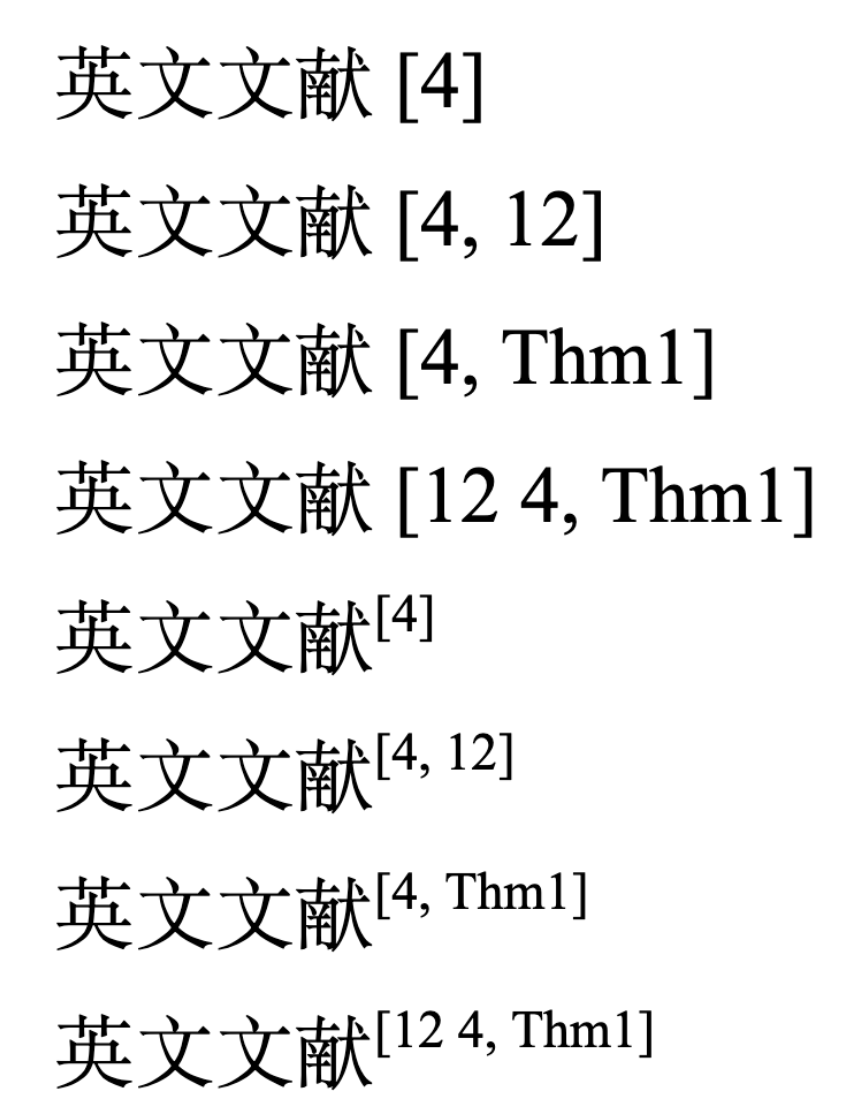
\includegraphics[width = 0.4\textwidth]{cite-parencite效果.png}
  \caption{\tn{cite} 和 \tn{parencite} 的效果}
  \label{figure:cite-parencite效果}
\end{figure}


\paragraph{定理类环境}


\begin{function}{axiom,counterexample,claim,corollary,conjecture,definition,example,lemma,property,proof,proposition,question,remark,theorem}
  \begin{ccnusyntax}[emph={[2]proof}]
    \begin{proof}(*\oarg{小标题}*)
      (*\meta{证明过程}*)
    \end{proof}
  \end{ccnusyntax}
  一系列预定义的数学环境。具体含义见表~\ref{tab:theorem}。
\end{function}

\begin{table}[ht]
  \caption{预定义的数学环境} \label{tab:theorem}
  \centering
  \small
  \begin{tblr}{
    width = \textwidth,
    columns = {c},
    hline{1,2,Z} = {solid}
  }
    \textbf{名称} &
      \env{axiom} & \env{counterexample} & \env{claim} & \env{corollary} & \env{conjecture} & \env{definition} & \env{example} \\
    \textbf{含义} &
      公理 & 反例 & 断言 & 推论 &
      猜想 & 定义 & 例 \\
  \end{tblr}

  \medskip

  \begin{tblr}{
    width = \textwidth,
    columns = {c},
    hline{1,2,Z} = {solid}
  }
    \textbf{名称} &
      \env{lemma} & \env{property} & \env{proof} & \env{proposition} & \env{question} & \env{remark} & \env{theorem} \\
    \textbf{含义} &
      引理 & 性质 & 证明 & 命题 &
      问题 & 注  & 定理 \\
  \end{tblr}
\end{table}

\begin{function}{\qedhere}
  证明环境(\env{proof})的最后会添加证毕符号“$\square$”。对于证明如果以公式结尾或其它某些情况时“$\square$”可能会出现在新的空白行的行尾,如果想要“$\square$”出现在“有内容的”行尾,可以在想要出现的地方使用 \tn{qedhere} 命令。
\end{function}

比如您可以在模版中测试下面代码查看效果:

\begin{latexexample}
  \begin{proof}
    \[
      x^2
    \]
  \end{proof}
  \begin{proof}
    \[
      x^2  \qedhere
    \]
  \end{proof}
\end{latexexample}


\begin{function}[added = 2022-06-04]{\ccnunewtheorem,\ccnunewtheorem*}
  \begin{ccnusyntax}[deletetexcs={\ccnunewtheorem,\ccnunewtheorem*},morekeywords={\ccnunewtheorem,\ccnunewtheorem*}]
    \ccnunewtheorem(*\oarg{计数器样式设置}\marg{环境中文名称}\marg{环境名}*)
    \ccnunewtheorem*(*\oarg{计数器样式设置}\marg{环境中文名称}\marg{环境名}*)
  \end{ccnusyntax}
  自定义定理类环境的命令。带星号的表示新定义的环境无计数器,类似于 \env{proof} 环境。
\end{function}

该命令的主要用法有下面四种:
\begin{latexexample}
  \ccnunewtheorem{测试}{test}
  \ccnunewtheorem*{测试试}{testt}
  \ccnunewtheorem[sibling = theorem]{测试试试}{testtt}
  \ccnunewtheorem[within = chapter]{测试试试试}{testttt}
\end{latexexample}

\begin{itemize}
  \item |\ccnunewtheorem{测试}{test}| 定义了一个 \env{test} 环境,label 名为 \env{测试}。环境自己用自己的计数器,并且跨 chapter 连续编号
  \item |\ccnunewtheorem*{测试试}{testt}| 定义了一个 \env{testt} 环境,label 名为 \env{测试试}。环境不编号。
  \item |\ccnunewtheorem[sibling = theorem]{测试试试}{testtt}| 定义了一个 \env{testtt} 环境,label 名为 \env{测试试试}。环境和 theorem 环境共用一个计数器。
  \item |\ccnunewtheorem[within = chapter]{测试试试试}{testttt}| 定义了一个 \env{testttt} 环境,label 名为 \env{测试试试试}。环境计数器的值和章节有关,形如 $x.y$,$x$ 表示章节的计数器的值,子计数器 $y$ 随新章节清零重新计数。
\end{itemize}

您可以看图~\ref{figure:ccnunewtheorem} 的效果来更好地理解四种用法的效果,

\begin{figure}[htbp]
  \centering
  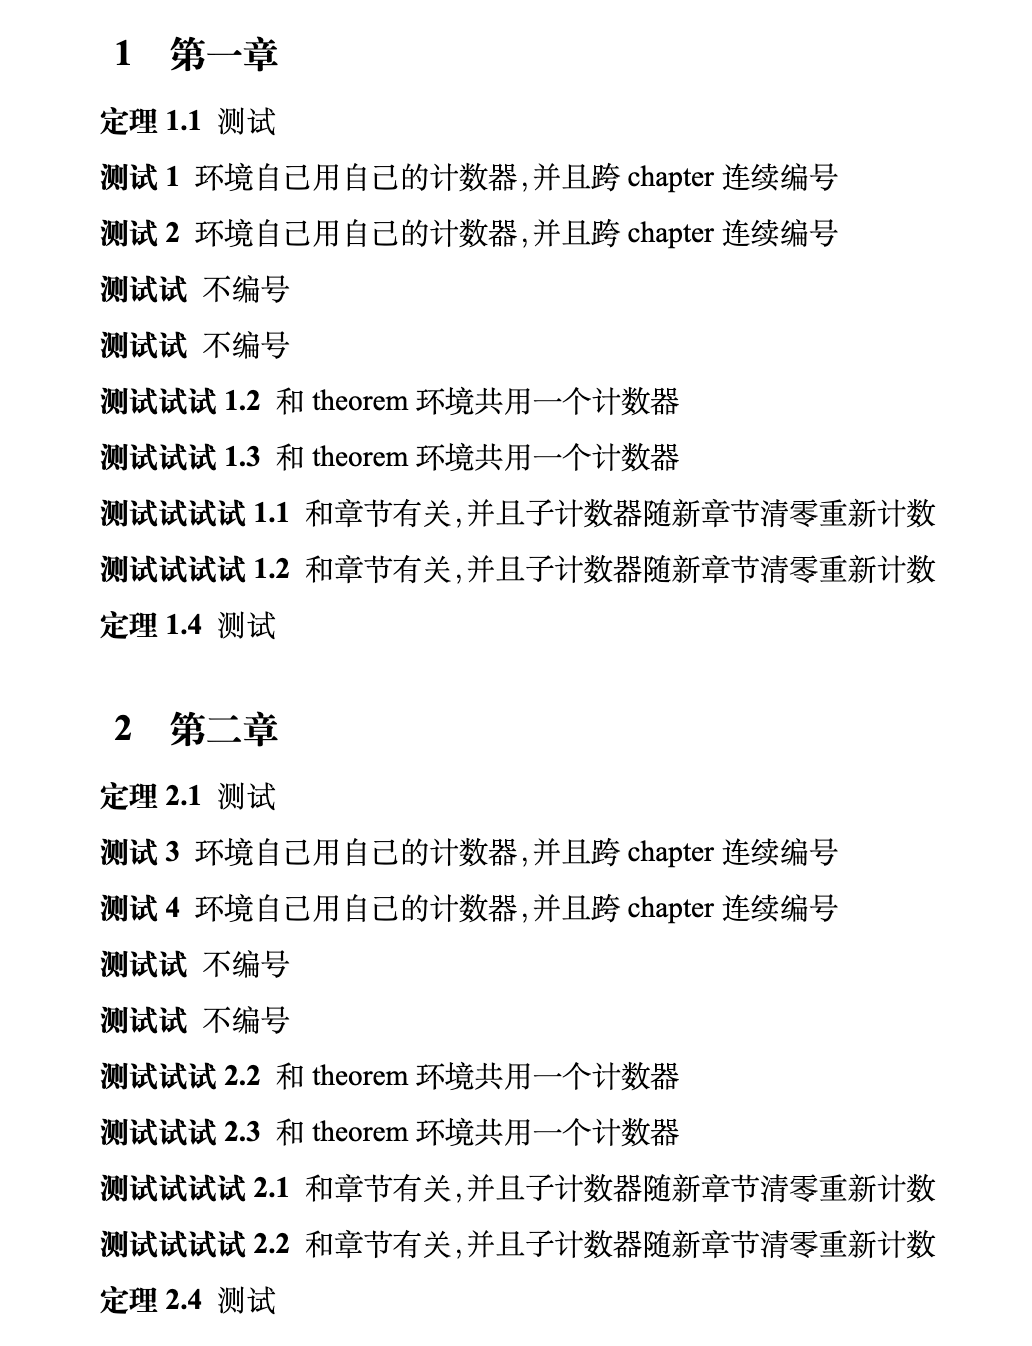
\includegraphics[width = 0.7\textwidth]{ccnunewtheorem.png}
  \caption{\tn{ccnunewtheorem} 示例}
  \label{figure:ccnunewtheorem}
\end{figure}



\subsubsection{豹尾}

\begin{function}{\backmatter}
  声明后置部分开始。
\end{function}

后置部分包含参考文献、声明页等。

\begin{function}{\printbibliography}
  \begin{ccnusyntax}[morekeywords={\printbibliography}]
    \printbibliography(*\oarg{选项}*)
  \end{ccnusyntax}
  打印参考文献列表。该命令由 \pkg{biblatex} 宏包直接提供,可用选项请参阅其文档。
\end{function}

\begin{function}{\acknowledgements}
  开启致谢章节。

\begin{latexexample}
  % acknowledgements.tex
  \acknowledgements
  
  <致谢内容>
\end{latexexample}
\end{function}


\begin{function}{\appendix}
  开启附录章节。
  
\begin{latexexample}
  % appendix.tex
  \appendix
  
  \chapter{<附录标题>}
  <附录内容>

  \chapter{<附录标题>}
  <附录内容>
\end{latexexample}

  附录和正文的章节层级相同,也是 \tn{chapter} 开始。需注意:\emph{硕博模版的附录在致谢前,本科模版的附录在致谢后。}

  根据 \parencite{研究生院研究生学位论文规范} 的要求“附录另起一页,“附录”两字居中,中间空两格,三号黑体加粗。如有多个附录,可用附录1、附录2区别并加以排序。” 模版已经做了自动化处理,即
  \begin{itemize}
    \item 如果 \file{appendix.tex} 中只有一个 \tn{chapter}\marg{内容} 的话,章节标题和目录中显示“附录 \meta{内容}”
    \item 如果 \file{appendix.tex} 中有两个及两个以上的 \tn{chapter}\marg{内容} 的话,章节标题和目录中显示“附录A \meta{内容}”、“附录B \meta{内容}”
  \end{itemize}
  但和一般的交叉引用不同,附录的此自动化处理,一般来说可能需要编译两次甚至三次,这个取决于用户在何时进行编译(比如编译之后又写了一个 \tn{chapter}\marg{内容} 的话,就需要三次编译才可以达到正确的章节标题和目录内容),但是三次(只要附录外的内容没问题,附录内没有报错)一定可以达到正确的编译效果。
\end{function}


\begin{function}{\publication}
  开启“攻读学位期间取得的研究成果”章节。此章节只有博士模版需要,只需要取消 \file{main.tex} 中的
\begin{latexexample}
  % % !TeX root = ../main.tex
\publication


\begin{publications}
  \item test
  \item test
  \item test
  \item test
  \item test
  \item test
  \item test
  \item test
  \item test
  \item test
  \item test
  \item test
  \item test
  \item test
  \item test
  \item test
\end{publications}
\end{latexexample}
  的代码注释,并且在 \file{publications.tex} 文件中输入相应内容即可。
\end{function}

\begin{function}{publications}
  \begin{ccnusyntax}[emph={[2]publications}]
    \begin{publications}
      \item (*\meta{研究成果1}*)
      \item (*\meta{研究成果2}*)
      ...
    \end{publications}
  \end{ccnusyntax}
  研究成果列表环境。研究成果的格式等需要用户自行输入,无法像参考文献一样自动化,具体的字体字样等命令请自行查阅 \href{https://ctan.math.illinois.edu/info/lshort/chinese/lshort-zh-cn.pdf}{lshort-zh-cn}。
\end{function}

\begin{function}{choices}
  \begin{ccnusyntax}[emph={[2]choices}]
    \begin{choices}(*\oarg{可选参数}*)
      \item (*\meta{选项1}*)
      \item (*\meta{选项2}*)
      ...
    \end{choices}
  \end{ccnusyntax}
  选项排版环境。对于有排版试卷、问卷等需求的用户,此环境能方便地帮您进行任意个选项的排版,并可以方便地调整选项 label 的样式。
\end{function}

用法和列表环境相同,使用 \tn{item} 分隔选项。label 的样式支持

\begin{itemize}
  \item arabic(阿拉伯数字)
  \item alph(小写英文)
  \item Alph(大写英文)
  \item roman(小写罗马数字)
  \item Roman(大写罗马数字)
  \item circlednumber(带圈数字)
\end{itemize}

如
\begin{latexexample}
  \begin{choices}[label = \arabic*)]
    \item 选项1
    \item 选项2
    \item 选项3
    \item 选项4
  \end{choices}
  
  \begin{choices}[label = (\alph*]
    \item 选项1
    \item 选项2
    \item 选项3
    \item 选项4
  \end{choices}
  
  \begin{choices}[label = \Alph*.]
    \item 选项1
    \item 选项2
    \item 选项3
    \item 选项4
  \end{choices}
  
  \begin{choices}[label = \roman*:]
    \item 选项1
    \item 选项2
    \item 选项3
    \item 选项4
  \end{choices}
  
  \begin{choices}[label = \Roman*-]
    \item 选项1
    \item 选项2
    \item 选项3
    \item 选项4
  \end{choices}
  
  \begin{choices}[label = \circlednumber*]
    \item 选项1
    \item 选项2
    \item 选项3
    \item 选项4
    \item 选项5
    \item 选项6
    \item 选项7
    \item 选项8
  \end{choices}
\end{latexexample}


还可以修改 \opt{columns} 键值来决定每行排多少个
\begin{latexexample}
  \begin{choices}[
    columns = 3,            % 手动控制每行多少个选项,否则自己根据宽度自动排版
    label   = (\arabic*)      % label 的样式,支持 arabic, alph, Alph, roman, Roman, circlednumber
  ]
    \item 选项1
    \item 选项2
    \item 选项3
    \item 选项4
    \item 选项5
    \item 选项6
  \end{choices}
\end{latexexample}

具体效果可见~\ref{figure:choices环境示例}。更多关于 \env{choices} 环境的精细调整可以查看 \url{https://gitee.com/zepinglee/exam-zh}。

\begin{figure}[htbp]
  \centering
  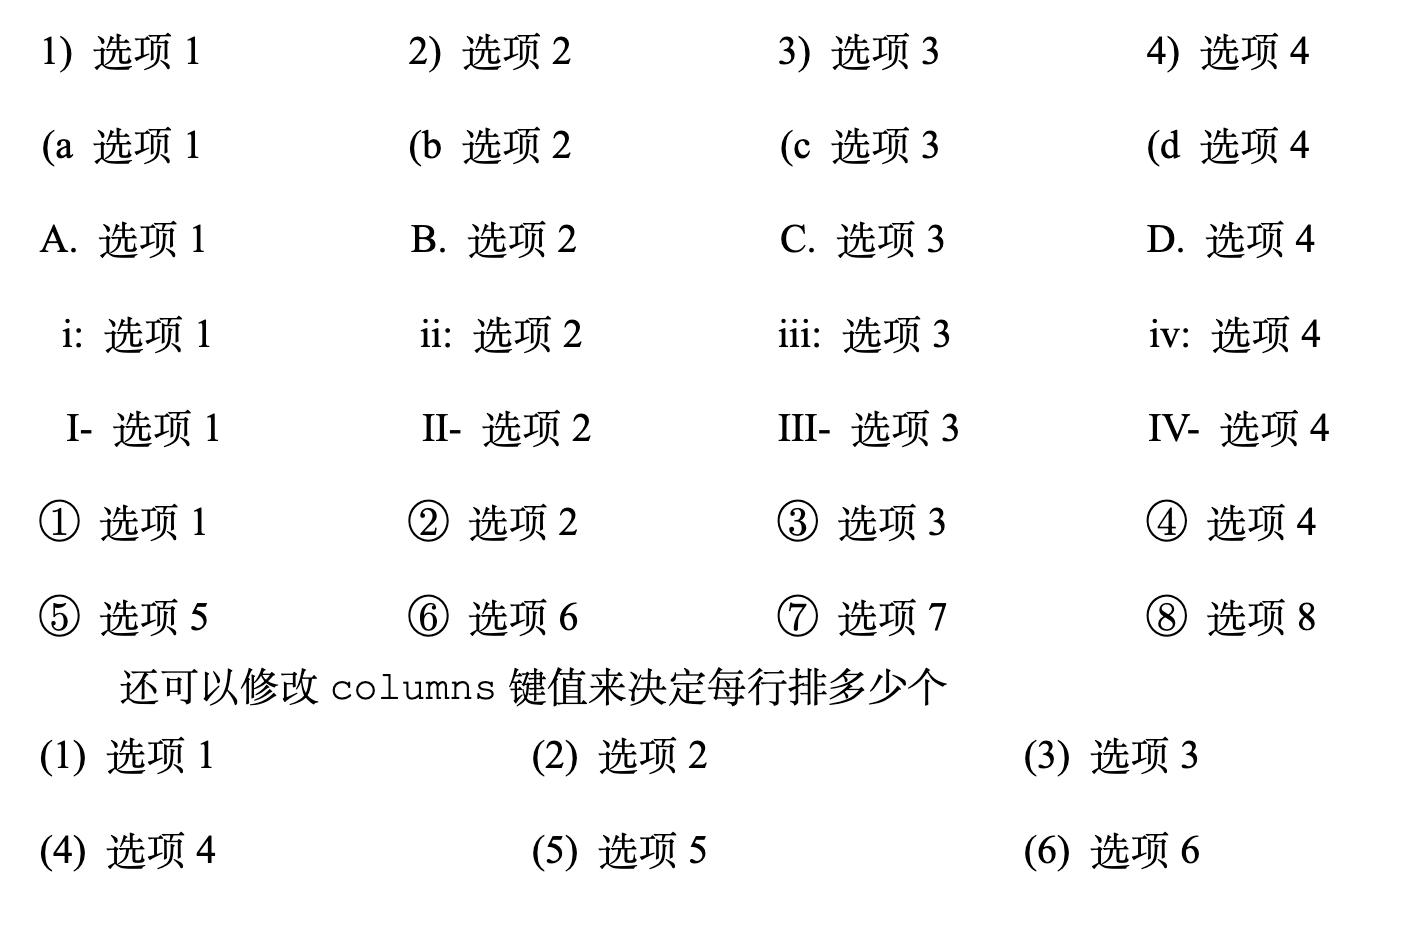
\includegraphics[width = 0.9\textwidth]{choices环境.png}
  \caption{\env{choices} 环境示例}
  \label{figure:choices环境示例}
\end{figure}





\section{宏包依赖情况}

使用不同编译方式、指定不同选项,会导致宏包依赖情况有所不同。
具体如下:
\begin{itemize}
  \item 在任何情况下,本模板都会\emph{显式}调用以下宏包
    (或文档类):
    \begin{itemize}
      \item \pkg{l3keys2e},用于扩展 \LaTeX3 编程环境。它们属于 \pkg{l3packages} 宏集。
      \item \cls{ctexbook},提供中文排版的通用框架。属于 \CTeX{} 宏集 。
      \item \pkg{geometry},用于调整页面尺寸。
      \item \pkg{fancyhdr},处理页眉页脚。
      \item \pkg{footmisc},处理脚注。
      \item \pkg{graphicx},提供图形插入的接口。
      \item \pkg{caption},用于设置题注。
      \item \pkg{fontspec},设置字体及字号。
      \item \pkg{tikzpagenodes},封面、扉页元素定位。
      \item \pkg{tabularray},表格宏包。
      \item \pkg{calc},提供 \tn{settototalheight} 等命令处理封面下划线。
      \item \pkg{etoolbox},给命令环境打补丁。
      \item \pkg{amsthm}、\pkg{thmtools},提供定理类环境设置接口。
      \item \pkg{xeCJKfntef},提供个人信息的下划线。
      \item \pkg{enumitem},列表环境相关设置。
      \item \pkg{tocloft},目录修改。
      \item \pkg{newtxmath} 和 \pkg{unicode-math},如果 \kvopt{style/font}{newtx} 或 \kvopt{style/font}{times} 则加载前者,其余选项则载入后者。后者对 \LaTeX 的数学排版功能进行了全面扩展。属于 \AmSLaTeX 套件
      \item  \pkg{biblatex},并依赖 \biber{} 程序。参考文献样式由\pkg{biblatex-gb7714-2015} 宏包提供。
      \item \pkg{hyperref},提供交叉引用、超链接、电子书签等功能。
    \end{itemize}
  \item 开启 \kvopt{style/footnote-style}{pifont} 后,会调用
    \pkg{pifont} 宏包。它属于 \pkg{psnfss} 套件。
\end{itemize}

这里只列出了本模板直接调用的宏包。这些宏包自身的调用情况,此处不再具体展开。如有需要,请参阅相关文档。



\section{CCNUthesis: TODO}


\begin{itemize}
  \item 手册本身
    \begin{itemize}
      \item 把 manual 中有用的部分写进 wiki 或手册
      \item “如何提问”
      \item 参考文献
    \end{itemize}
  \item wiki
    \begin{itemize}
      \item 问题解决
        \begin{itemize}
          \item 如果是 author-year 的时候,对于多音字怎么办?——加 key
          \item 标题中一些宏如果报错:\tn{texorpdfstring}
        \end{itemize}
      \item 学习其它模版的 wiki
      \item 重新整理 wiki,并和手册进行取舍合并
        \begin{itemize}
          \item \TeXLive 安装细节
          \item VScode
        \end{itemize}
      \item 提供一些示例
        \begin{itemize}
          \item tabularray
          \item physicx
          \item fixdif
          \item choices
        \end{itemize}
    \end{itemize}
  \item 学习其它论文模版的处理
    \begin{itemize}
      \item thuthesis
      \item sjtuthesis
      \item ucasthesis
      \item ustcthesis
      \item cquthesis
      \item njuthesis
      \item hithesis
    \end{itemize}
  \item 录制新的讲解视频
\end{itemize}


\printbibliography

\end{document}